\documentclass[12pt,a4paper]{article}
\usepackage{geometry}
\usepackage[numbers]{natbib}
\usepackage{amssymb, amsmath}
\usepackage{graphicx}
\usepackage{grffile}
\graphicspath{{../Figures/}}
\usepackage{gensymb}
\usepackage[font=small]{caption}
\usepackage[utf8]{inputenc}
\usepackage[english]{babel}
\usepackage{fancyhdr}
\usepackage[raggedright]{titlesec}
\usepackage{subcaption}
\usepackage{multirow}
\usepackage{dirtytalk}
\usepackage{framed}
\usepackage[pdftex,breaklinks]{hyperref}
\hypersetup{
  colorlinks   = true, %Colours links instead of ugly boxes
  urlcolor     = green, %Colour for external hyperlinks
  linkcolor    = blue, %Colour of internal links
  citecolor   = red %Colour of citations
}


\begin{document}
\author{Katrina Ashton}


\pagestyle{fancy}
\fancyhf{}
\rhead{\thepage}
\lhead{u5586882}

\section{What I've done}
\begin{itemize}
\item{Testing RealSense camera}
\end{itemize}

\section{Parts of report to look at}
\begin{itemize}
\item{Nothing changed since last week}
\end{itemize}

\section{Questions}
\begin{itemize}
\item{}
\end{itemize}

\section{Comments}
\begin{itemize}
\item{It seems like Alex is working on the cables. I was going to send him an email reminding him on Friday but he sent me and Jean-Luc one asking for specifications for one of the cables (which Jean-Luc gave him). He also had my RealSense camera and TX2 (at least I certainly hope he has it, as it wasn't on my desk).}
\item{I need to submit a mid-semester report on the 25th (only a few pages summarizing what I've done, etc.)}
\end{itemize}

\section{Testing RealSense with Vicon}
\textbf{Set-up} \\
The RealSense camera is set-up pointing at a number of objects lying on the ground of the flying space. It is positioned in the groove of the white box. It stays relatively still but both the box and the RealSense itself are sensitive to bumps.
\\\\
The RealSense is connected to the TX2 (with orbitty board), and then SSHed to via an Ethernet cable. 
\\\\
\textbf{Method} \\
The camera remains still while point clouds are captured for about 5 seconds. The data collection program is then stopped. 
\\\\
For some reason the code wasn't letting the data collection program be re-run through SSH after it was canceled without restarting the TX2 (I did not have this issue with the TX1 which I connected to directly). Thus the TX2 was restarted by disconnecting and reconnecting the power (taking care not to bump the camera). Before the power was reconnected, the SD card was also removed from the TX2 and inserted into a laptop. The captured pointclouds were moved to a separate folder so that it would be clear under which conditions they were captured.
\\\\
The Vicon system was then activated and the above procedure repeated (but without reconnecting the power for the TX2 at the end).
\\\\
\textbf{Results} \\
	\begin{figure}[h]
		\centering
		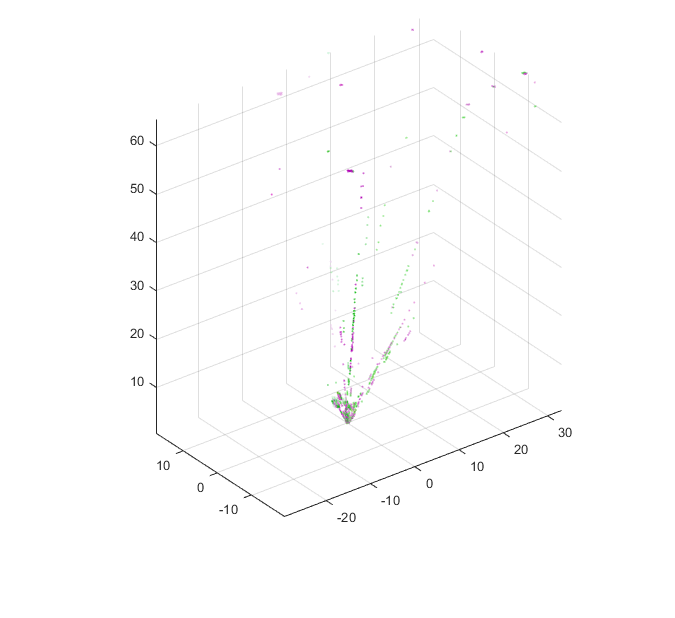
\includegraphics[height=50mm, trim = 20mm 20mm 20mm 20mm, clip]{first_frame_compare.png}
		\caption{Comparison of first point cloud with (green) and without (purple) Vicon on. Registering the point clouds gives $\alpha = 0.1104, \beta = -2.2856, \gamma = 2.5918$ with rmse 0.5990.}
		\label{f: vicon first frame}
	\end{figure}

	\begin{figure}[h]
		\centering
		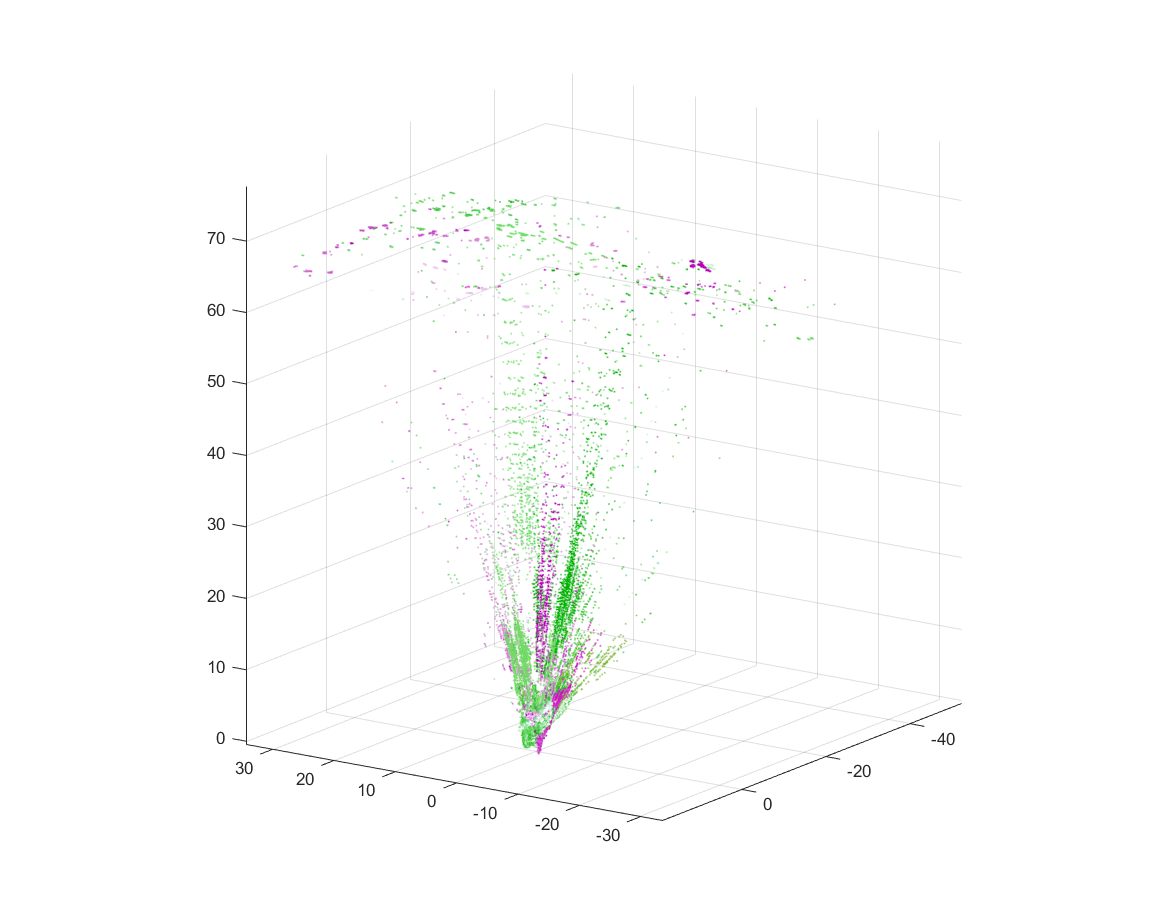
\includegraphics[height=50mm, trim = 20mm 20mm 20mm 20mm, clip]{full_compare.png}
		\caption{Comparison of registered point clouds with (green) and without (purple) Vicon on. Registering the point clouds gives $\alpha = 0.0012, \beta = 0.5442, \gamma = -0.5174$ with rmse 0.4770.}
		\label{f: vicon all frame}
	\end{figure}

\newpage
\section{Testing RealSense for different movement speeds}
\textbf{Set-up} \\
Two strips of tape are placed on the (straight) edge of a desk about 60cm apart.
\\\\
The RealSense is connected to the TX2 (with orbitty board), and then SSHed to via an Ethernet cable. 
\\\\
\textbf{Method} \\
Camera is held with the end at the edge of the left piece of tape, sitting on the edge of the table. The data capture program is started while the camera is held still for 4 seconds (letting the exposure, etc. settle). The camera is then moved at a slow speed along the edge of the table to the other end of the tape, after which the data capture program is immediately canceled. The camera was moved by hand, so there was likely variation in the movement speed.
\\\\
As with the Vicon test, the TX2 had to be restarted between tests. The data was also moved to a separate folder after each test.
\\\\
The above was repeated with medium-speed camera movement and then again with fast movement.
\\\\
\textbf{Results} \\
	\begin{figure}[h]
		\centering
		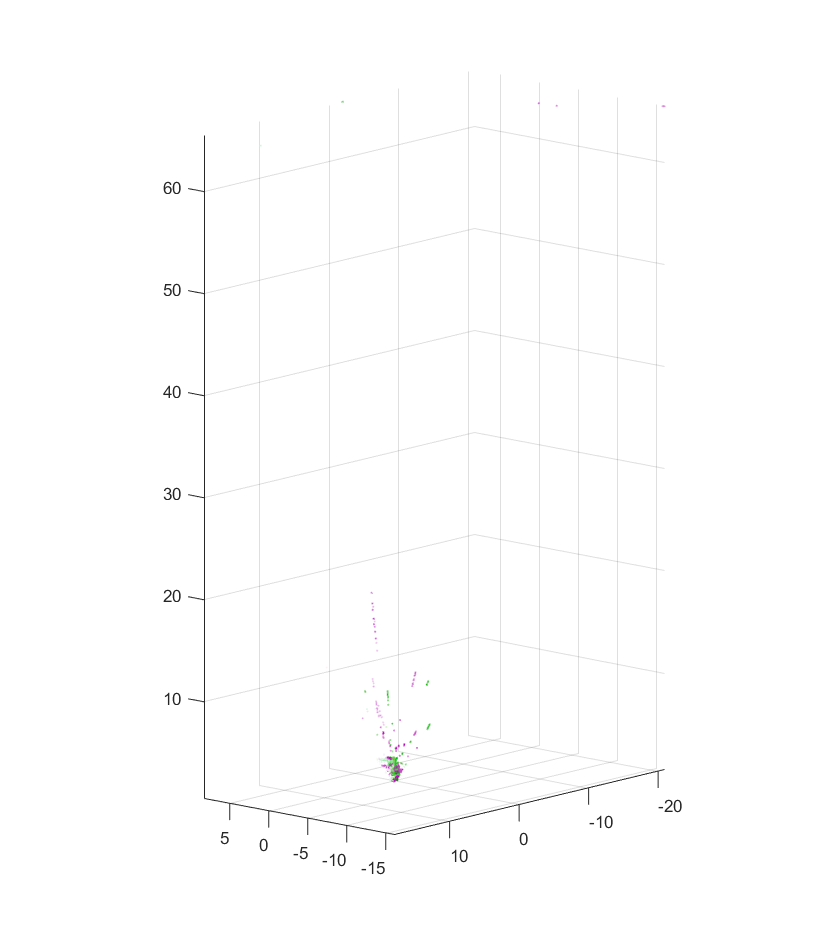
\includegraphics[height=50mm, trim = 20mm 10mm 20mm 140mm, clip]{slow_med.png}
		\caption{Comparison of middle point cloud for a camera that is moving slowly (green) and at a medium speed (purple). Registering the point clouds gives $\alpha = 0.2751, \beta = -2.5075, \gamma = 2.6075$ with rmse 0.2146.}
		\label{f: slow v med}
	\end{figure}

	\begin{figure}[h]
		\centering
		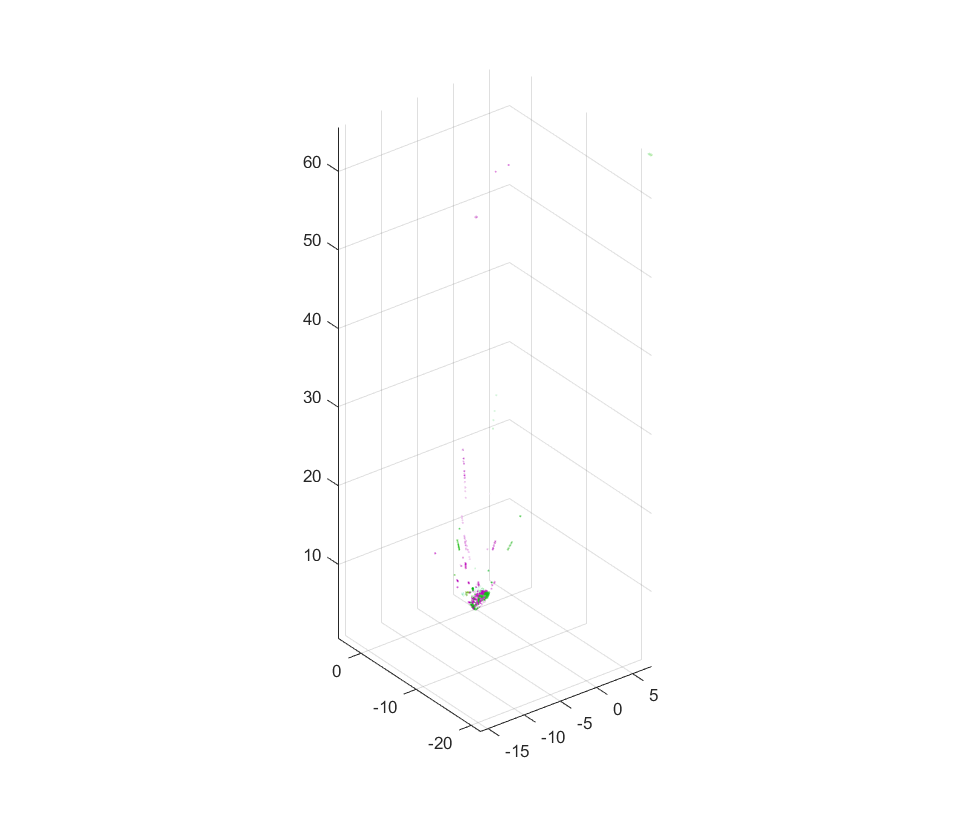
\includegraphics[height=50mm, trim = 20mm 10mm 20mm 100mm, clip]{slow_fast.png}
		\caption{Comparison of middle point cloud for a camera that is moving slowly (green) and quickly (purple). Registering the point clouds gives $\alpha = 0.2128, \beta = 2.7353, \gamma = -2.8896$ with rmse 0.1690.}
		\label{f: slow v med}
	\end{figure}

\end{document}